\documentclass[a4j]{jarticle}
\usepackage[dvipdfmx]{graphicx}	%必要
\usepackage[dvipdfmx]{color}	%必要
\usepackage{url}				%実験のテンプレに記載

\setlength{\headsep}{-5mm}
\setlength{\oddsidemargin}{0mm}
\setlength{\textwidth}{165mm}
\setlength{\textheight}{230mm}
\setlength{\footskip}{20mm}


\begin{document}
\appendix
\section{付録}
図\ref{全体}, \ref{成長記録}, \ref{ゲーム}, \ref{SNS}は本システムのユースケース図を示しています。

\begin{figure}[h]
  \begin{center}
    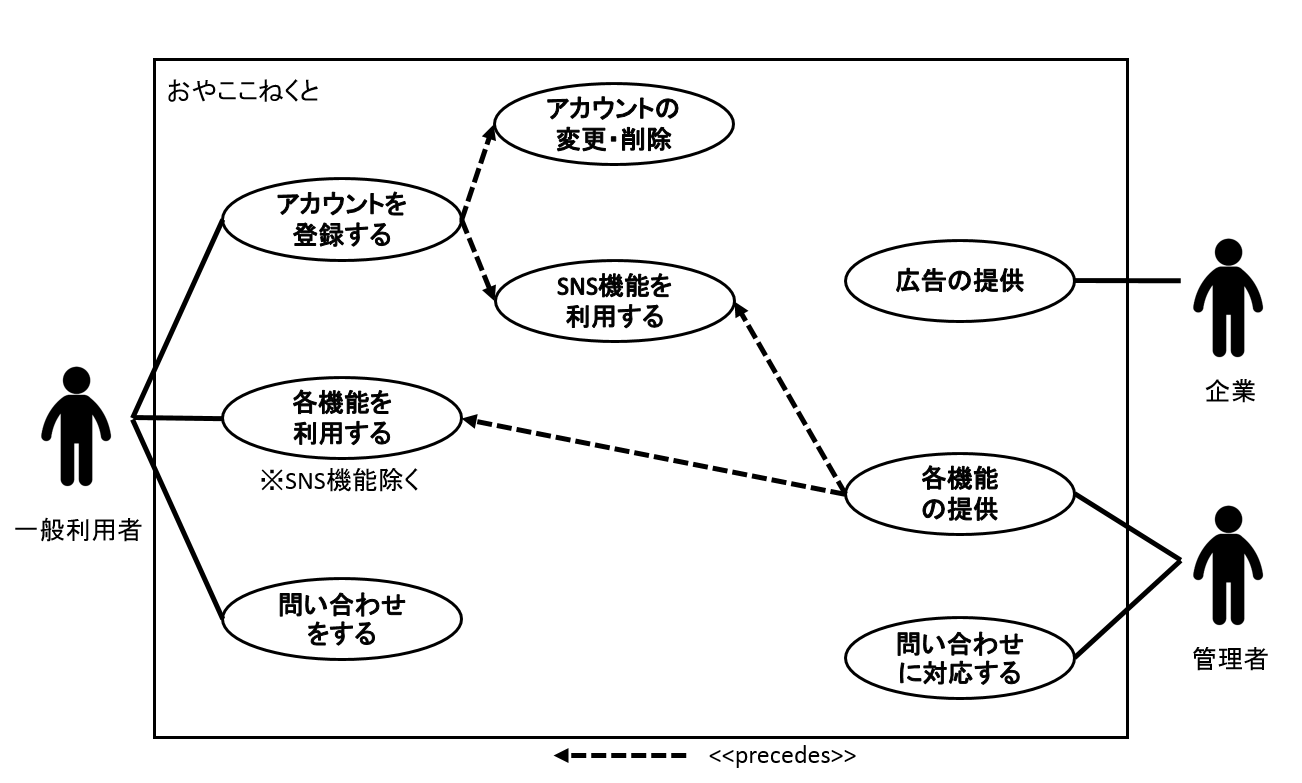
\includegraphics[width = 14cm, height = 7cm]{付録_全体.png}
    \caption{システム全体のユースケース図}
    \label{全体}
  \end{center}
\end{figure}

\begin{figure}[h]
  \begin{center}
    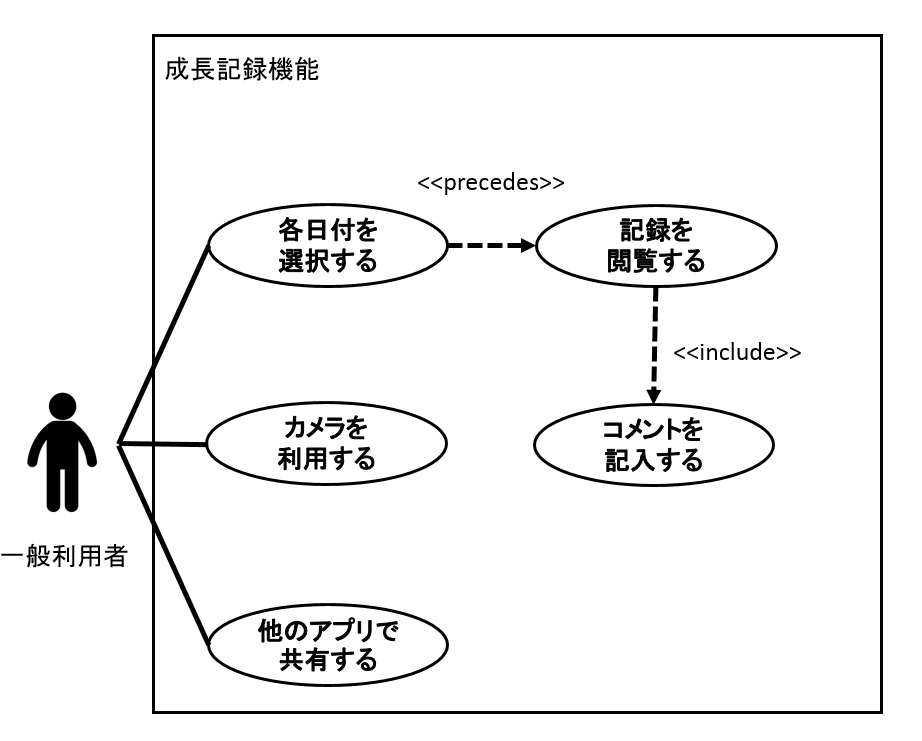
\includegraphics[width = 14cm, height = 7cm]{付録_成長記録.png}
    \caption{成長記録機能のユースケース図}
    \label{成長記録}
  \end{center}
\end{figure}

\begin{figure}[h]
  \begin{center}
    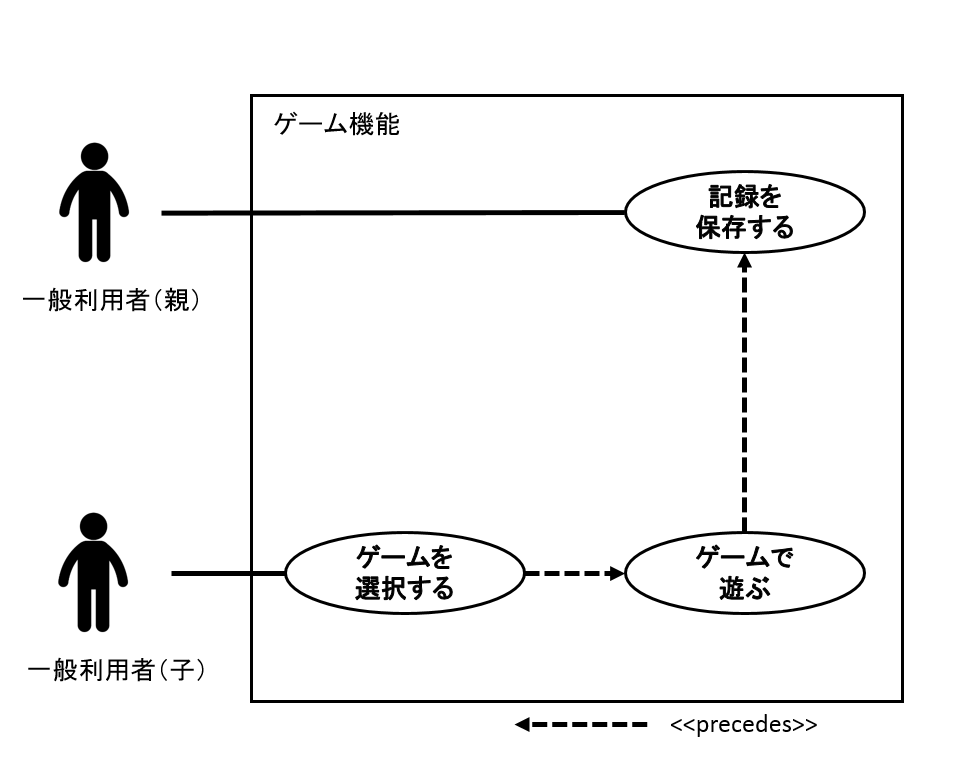
\includegraphics[width = 14cm, height = 7cm]{付録_ゲーム.png}
    \caption{ゲーム機能のユースケース図}
    \label{ゲーム}
  \end{center}
\end{figure}

\begin{figure}[h]
  \begin{center}
    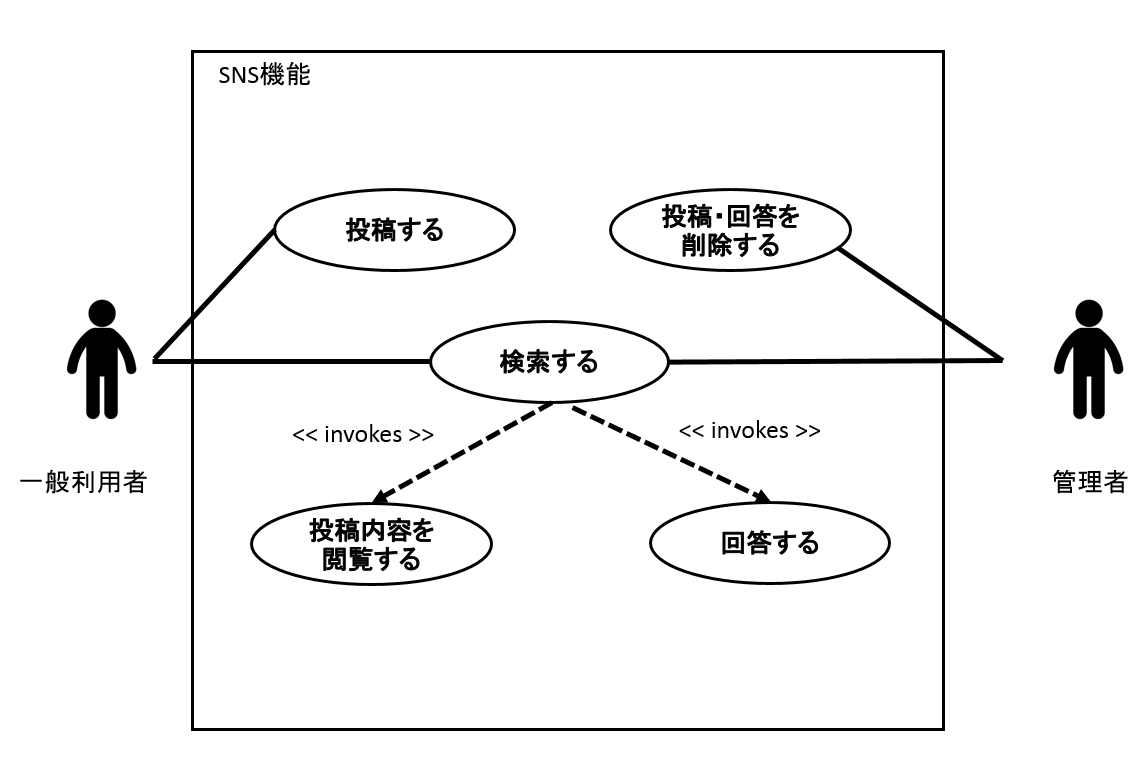
\includegraphics[width = 14cm, height = 7cm]{付録_sns.png}
    \caption{SNS機能のユースケース図}
    \label{SNS}
  \end{center}
\end{figure}


\end{document}

